\documentclass[11pt]{article}
\usepackage{amsmath, amsfonts, amsthm, amssymb}  % Some math symbols
\usepackage[utf8x]{inputenc}
\usepackage{fullpage}
\usepackage[x11names, rgb]{xcolor}
\usepackage{graphicx}
\usepackage{tikz}
\usepackage{etoolbox}
\usepackage{enumerate}
\usepackage{enumitem}
\usepackage{listings}
\usepackage{hyperref}
\usepackage{lipsum}
\usepackage{sectsty}
\usepackage{verbatim}
\usetikzlibrary{decorations,arrows,shapes}

%% Define the title contents
\title{CSE 311 - HW 1}
\author{Eric Boris \newline with Maxime Sutters, Brittan Robinett, Micah Witthaus}
\date{September 2019}

%% Left align the title 
\makeatletter
\renewcommand{\maketitle}{\bgroup\setlength{\parindent}{0pt}
\begin{flushleft}
  \textbf{\@title}

  \@author
  
  \@date
\end{flushleft}\egroup
}
\makeatother

%% Set the size of the section header
\sectionfont{\fontsize{11}{12}\selectfont}

%% Set the size and format of the subsection header
\subsectionfont{\fontsize{11}{12}\selectfont}
\renewcommand{\thesubsection}{\thesection (\alph{subsection})}

%%--- Begin the Document ---%%

\begin{document}
\maketitle

\section{} %% Problem 1
\subsection{} %% 1.a
\begin{align*}
	f &: \text{The stadium is full.} \\
	c &: \text{The crowd is subdued.} \\
	w &: \text{We will win the game.} \\
	&: (f \land \neg{c}) \rightarrow w
\end{align*}
	
\begin{comment}
\begin{center}
\begin{tabular}{ c|c|c|c|c|c } 
	f & c & w & $\neg{c}$ & $(f \land \neg{c})$ & $(f \land \neg{c}) \rightarrow w$ \\
	\hline
	T & T & T & F & F & T \\
	T & T & F & F & F & T \\
	T & F & T & T & T & T \\
	T & F & F & T & T & F \\
	F & T & T & F & F & T \\
	F & T & F & F & F & T \\
	F & F & T & T & F & T \\
	F & F & F & T & F & T \\
\end{tabular}
\end{center}
\end{comment}

\subsection{} %% 1.b
\begin{align*}
	w &: \text{The watch is more than \$25.} \\
	s &: \text{The watch is on sale.} \\
	b &: \text{I will buy the watch.} \\
	i) &: b \rightarrow \neg{w}    \\
	ii) &: \neg{b} \rightarrow \neg{s} \\
	iii) &: b \rightarrow(s \land \neg{w})
\end{align*}

\subsection{} %% 1.c
\begin{align*}
	e &: \text{The stack is empty.} \\
	f &: \text{The stack is full.} \\
	u &: \text{You can push onto the stack.} \\
	o &: \text{You can pop from the stack.} \\
	i) &: e \rightarrow (u \land \neg{o}) \\
	ii) &: (\neg{u} \land o) \rightarrow f \\
	iii) &: (\neg{u} \lor \neg{o}) \rightarrow (e \lor f)
\end{align*}

\section{} %% Problem 2
%% This is similar to an example from 11.3
We begin by writing a truth table for the possible combinations of p, q, r, and F(p,q,r). From that we see that there are four rows that produce the outcome we're looking for: 1, 2, 3, and 5. Grouping the states of p, q, and r in each of those 4 rows with "and" and then joining each of the groups with "or" yields a function that is true when a majority of the inputs are true.
\begin{center}
\begin{tabular}{ c|c|c|c } 
	p & q & r & F(p,q,r) \\
	\hline
	T & T & T & T \\
	T & T & F & T \\
	T & F & T & T \\
	T & F & F & F \\
	F & T & T & T \\
	F & T & F & F \\
	F & F & T & F \\
	F & F & F & F \\
\end{tabular}
\end{center}
\begin{center} 
$(p \land q \land r) \lor (p \land q \land \neg{r}) \lor (p \land \neg{q} \land r) \lor (\neg{p} \land q \land r) \rightarrow F(p,q,r)$
\end{center}

\section{} %% Problem 3
From the following truth table we see that the desired state of the circuit B(p,q,r) can be made to match a compound proposition, namely, it's last column. We then translate that into a circuit diagram by replacing logical symbols with circuit components. 
\begin{center}
\begin{tabular}{ c|c|c|c|c|c|c|c } 
	p & q & r & $\neg{p}$ & $\neg{q}$ & $\neg{r}$ & $B(p,q,r)$ & $(p \land q \land \neg{r}) \lor (p \land \neg{q} \land r) \lor (\neg{p} \land q \land r)$ \\
	\hline
	T & T & T & F & F & F & F & F \\
	T & T & F & F & F & T & T & T \\
	T & F & T & F & T & F & T & T \\
	T & F & F & F & T & T & F & F \\
	F & T & T & T & F & F & T & T \\
	F & T & F & T & F & T & F & F \\
	F & F & T & T & T & F & F & F \\
	F & F & F & T & T & T & F & F \\
\end{tabular}
\end{center}
\begin{figure}[h]
	\centering
	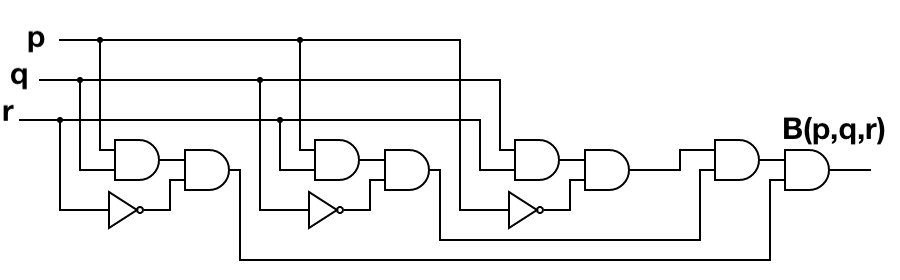
\includegraphics[scale=0.4]{CSE311HW1Diagram.png}
	\label{Circuit Diagram of B(p,q,r)}
	\caption{Circuit Diagram of B(p,q,r)}
\end{figure}

\section{} %% Problem 4

\subsection{} %% 4.a
\begin{center}
\begin{tabular}{ c|c|c } 
	p & $\neg{p}$ & $A(F,p) = F \lor \neg{p}$ \\
	\hline
	T & F & F \\
	T & F & F \\
	F & T & T \\
	F & T & T \\
\end{tabular}
\end{center}

\subsection{} %% 4.b
\begin{center}
\begin{tabular}{ c|c|c|c|c } 
	p & q & $(p \lor q)$& $A_{1}(F,q) = F \lor \neg{q}$ & $A_{2}(p,A_{1}) = p \lor \neg{A_1}$ \\
	\hline
	T & T & T & F & T \\
	T & F & T & T & T \\
	F & T & T & F & T \\
	F & F & F & T & F \\
\end{tabular}
\end{center}

\subsection{} %% 4.c
\begin{center}
\begin{tabular}{ c|c|c|c|c } 
	p & q & $\neg{(p \land q)}$ & $A_{1}(F,p) = F \lor \neg{p}$ & $A_{2}(A_1,q) = A_1 \lor \neg{q}$ \\
	\hline
	T & T & F & F & F \\
	T & F & T & F & T \\
	F & T & T & T & T \\
	F & F & T & T & T \\
\end{tabular}
\end{center}

\subsection{} %% 4.d
\begin{center}
\begin{tabular}{ c|c|c|c|c|c } 
	p & q & $(p \land q)$ & $A_{1}(F,p) = F \lor \neg{p}$ & $A_{2}(A_1,q) = A_1 \lor \neg{q}$ & $A_3(F,A_2) = F \lor \neg{A_2}$\\
	\hline
	T & T & T & F & F & T \\
	T & F & F & F & T & F \\
	F & T & F & T & T & F \\
	F & F & F & T & T & F \\
\end{tabular}
\end{center}

\section{} %% Problem 5
\subsection{} %% 5.a
By the last two columns of the truth table we see that the last three rows fail to agree. 
\begin{center}
\begin{tabular}{ c|c|c|c|c } 
	p & q & $(p \land q)$ & $p \lor (p \land q)$ & $q \lor (p \land q)$ \\
	\hline
	T & T & T & T & T \\
	T & F & F & T & F \\
	F & T & F & F & T \\
	F & F & F & F & F \\
\end{tabular}
\end{center}

\subsection{} %% 5.b
By the last two columns of the truth table we see that none of the rows agree.
\begin{center}
\begin{tabular}{ c|c|c|c|c|c|c } 
	p & q & $\neg{p}$ & $\neg{q}$ & $(p \oplus q)$ & $\neg{(p \oplus q)}$ & $\neg{p} \oplus \neg{q}$ \\
	\hline
	T & T & F & F & F & T & F \\
	T & F & F & T & T & F & T \\
	F & T & T & F & T & F & T \\
	F & F & T & T & F & T & F \\
\end{tabular}
\end{center}

\subsection{} %% 5.c
By the last two rows of the truth table we see that rows six and eight fail to agree.
\begin{center}
\begin{tabular}{ c|c|c|c|c|c|c } 
	p & q & r & $(q \rightarrow r)$ & $(p \rightarrow q)$ & $p \rightarrow (q \rightarrow r)$ & $(p \rightarrow q) \rightarrow r$ \\
	\hline
	T & T & T & T & T & T & T \\ 
	T & T & F & F & T & F & F \\
	T & F & T & T & F & T & T \\
	T & F & F & T & F & T & T \\
	F & T & T & T & T & T & T \\
	F & T & F & F & T & T & F \\
	F & F & T & T & T & T & T \\
	F & F & F & T & T & T & F \\
\end{tabular}
\end{center}

\subsection{} %% 5.d
By the last two rows of the truth table we see that the second and third rows fail to agree.
\begin{center}
\begin{tabular}{ c|c|c|c|c|c } 
	p & q & $(p \rightarrow q)$ & $(q \rightarrow p)$ & $(p \rightarrow q) \rightarrow (q \rightarrow p)$ & $(q \rightarrow p) \rightarrow (p \rightarrow q)$ \\
	\hline
	T & T & T & T & T & T \\
	T & F & F & T & T & F \\
	F & T & T & F & F & T \\
	F & F & T & T & T & T \\
\end{tabular}
\end{center}

\section{} %% Problem 6
\subsection{} %% 6.a 1.1 knights and knaves
We begin by defining the identities of the two people and whether the statement is true. The speaker can either be a student or a TA and the other person can also be either a student or a TA and the truth of the statement is dependent on the speaker's identity. ($s$ will always have the same truth value as $p$ but is retained for clarity.) 
\begin{align*}
	p &: \text{The speaker is a student.} \\
	q &: \text{The other person is a student.} \\
	s &: \text{At least one of them is a TA.}
\end{align*}
There are four possible cases of the identites of the people: neither person is a student, the speaker is a student and the other person isn't, the speaker isn't a student but the other person is, and both speaker and other person are students. Or, more formally:
\begin{align*}
	C1 &: \neg{p} \land \neg{q} \\
	C2 &: p \land \neg{q} \\
	C3 &: \neg{p} \land q \\
	C4 &: p \land q \\
\end{align*}
Let us now consider which, if any, of these cases are possible. 
\begin{center}
\begin{tabular}{ c|c|c|c|c } 
	p & q & s & $s \land [(\neg{p} \land q) \lor (p \land \neg{q}) \lor (\neg{p} \land \neg{q})]$ & $\neg{s} \land (p \land q)$ \\ 
	\hline
	T & T & T & F & F \\
	T & F & T & T & F \\
	F & T & F & F & F \\
	F & F & F & F & F \\
\end{tabular}
\end{center}
Let us consider the two possible cases of the speaker's identity. 

If the speaker is a student they are telling the truth and at least one of them is a TA. We already know that the speaker is a student so the only possible scenario is that the speaker is a student and the other person is a TA. 

If the speaker is a TA they are lying and neither is a TA, but that would be a contradiction. Therefore the only possibility is that the speaker is a student and the other person is a TA.

\subsection{} %% 6.b 
As above, we begin by defining propositions. 
\begin{align*}
	p &: \text{The speaker is a student.} \\
	q &: \text{The second person is a student.} \\
	r &: \text{The third person is a student.} \\
	s &: \text{Every TA in the circle has a TA to their immediate right.}
\end{align*}

For the spoken statement to be true, there are four possible states: the speaker is a student and the other people in the circle are also students (The statement is not false as it doesn't state that there \textit{are} TAs in the circle.) or the speaker is a TA, is lying, and there are no other TAs, or one of the other people is a TA. Notably, the state where all the people are TAs can't be true because then the statement would be true. (Truth table columns truncated for space.)
\begin{center}
\begin{tabular}{ c|c|c|c|c } 
	p & q & r & s & $(p \land q \land r \land s) \lor (\neg{p} \land q \land r \land \neg{s}) \lor (\neg{p} \land q \land \neg{r} \land \neg{s}) \lor (\neg{p} \land \land{q} \land r \land \neg{s})$\\
	\hline
	T & T & T & T & T \\
	T & T & F & T & F \\
	T & F & T & T & F \\
	T & F & F & T & F \\
	F & T & T & F & T \\
	F & T & F & F & T \\
	F & F & T & F & T \\
	F & F & F & F & F \\
\end{tabular}
\end{center}

\section{} %% Problem 7
We begin by XNORing $R_1$ and $R_2$ and store the result in $R_2$. Then, we XNOR $R_1$ and $R_2$ again and store the result in $R_1$. Finally, we XNOR $R_1$ and $R_2$ again and store the result in $R_2$. This has the effect of swapping the values as show by match between the last two rows of the step table and truth table. 
\begin{center}
\begin{tabular}{ c|c|c } 
	Steps & $R_1$ & $R_2$ \\
	\hline
	0 & p & q \\
	1 & p & $p \bar{\oplus} q$ \\
	2 & $(p \bar{\oplus} q) \bar{\oplus} p$ & $p \bar{\oplus} q$ \\
	3 & $(p \bar{\oplus} q) \bar{\oplus} p$ & $((p \bar{\oplus} q) \bar{\oplus} p) \bar{\oplus} (\bar{p \oplus q})$ \\
\end{tabular}
\end{center}
\begin{center}
\begin{tabular}{ c|c|c|c|c } 
	p & q & $p \bar{\oplus} q$ & $(p \bar{\oplus} q) \bar{\oplus} p$ & $((p \bar{\oplus} q) \bar{\oplus} p) \bar{\oplus} (\bar{p \oplus q})$ \\
	\hline
	T & T & T & T & T \\
	T & F & F & F & T \\
	F & T & T & F & F \\
	F & F & F & T & F \\
\end{tabular}
\end{center}


\end{document}